\chapter{Dise\~no e Implementaci\'on del prototipo}

% **************************** Define Graphics Path **************************
\ifpdf
    \graphicspath{{Chapter4/Figs/Raster/}{Chapter4/Figs/PDF/}{Chapter4/Figs/}}
\else
    \graphicspath{{Chapter4/Figs/Vector/}{Chapter4/Figs/}}
\fi

Este cap\'itulo esta destinado a la comprensi\'on de los aspectos principales que hacen al dise\~no e implementaci\'on del prototipo para la nueva red aca\'emica. Cabe destacar que en el mismo se toman como punto de partida las decisiones asumidas en el cap\'itulo anterior.

\section{Aspectos generales}

Como se menciona en el estado del arte, de acuerdo al enfoque SDN, en la arquitectura OpenFlow se tienen los planos de datos y control. En la arquitectura de OpenFlow, el plano de control es implementado por un software de control o comúnmente llamado Controlador, y el plano de datos esta compuesto por los diferentes dispositivos de la red compatibles con OpenFlow.\\

La arquitetcura del prototipo, como puede apreciarse en la imagen ~\ref{fig:OpenSourceRArch0} se condice con esta estructura. Por un lado se tiene una red h\'ibrida IP/MPLS, donde cada nodo es un switch MPLS/Openflow híbrido, cuya arquitectura se definir\'a m\'as adelante; y por otro se tiene la entidad de control o Controlador sobre la cual se ejecuta la aplicaci\'on encargada de programar el comportamiento de cada uno de estos nodos. Finalmente, mediante el protocolo OpenFlow esta aplicaci\'on instala la configuraci\'on necesaria en cada nodo, para por ejemplo la implementaci\'on de un servicio de VPN particular.\\

\newpage
\begin{figure}[htbp!] 
\centering    
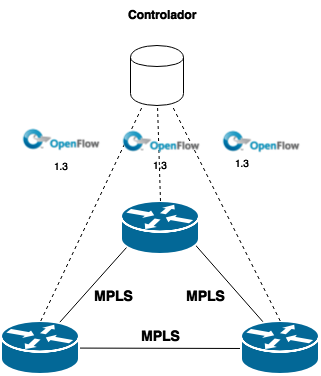
\includegraphics[width=0.4\textwidth]{Arch_Figure0}
\caption[OpenSourceRArch0]{Esquema general del prototipo}
\label{fig:OpenSourceRArch0}
\end{figure}

Se tienen entonces dos claras lineas de trabajo; el desarrollo del switch, de aquí en mas RAU-Switch y el desarrollo de la entidad Controlador. 

\section{RAU-Switch}
Cada nodo del prototipo es implementado por lo que en este trabajo se denomin\'o RAU-Switch; un switch MPLS/OpenFlow híbrido. Este switch se divide en diferentes componentes como se muestra en la figura~\ref{fig:OpenSourceRArch}.

\newpage
\begin{figure}[htbp!] 
\centering    
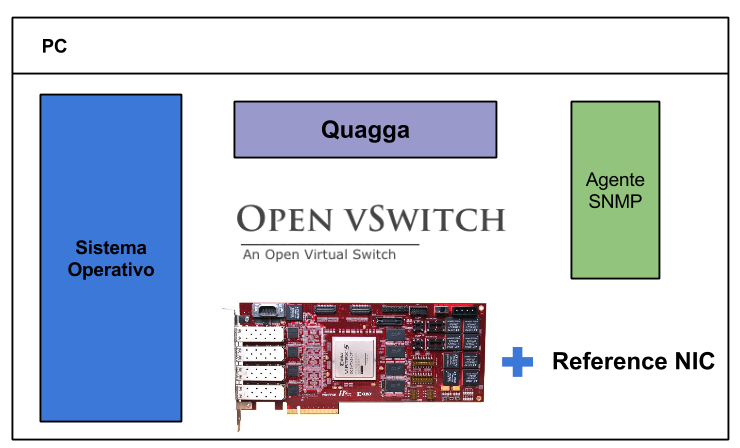
\includegraphics[width=0.7\textwidth]{Arch_Figure1}
\caption[RAU-Switch - diagrama de componentes]{RAU-Switch - diagrama de componentes}
\label{fig:OpenSourceRArch}
\end{figure}

\subsection{Plataforma de la PC}
El switch esta constru\'ido sobre la plataforma de una PC de escritorio convencional. En particular se trabaja con un procesador Intel Core i7 de 64 bits, una Mother ASUS ROG Maximus Formula VI, 16GB de memoria DDR3, y un disco HDD de 1TB de capacidad. En el apéndice \ref{C.1} pueden encontrarse estos detalles con mayor profundidad.

\subsection{Sistema Operativo}
Sobre el sistema operativo, se decidio trabajar con Ubuntu 12.04 sobre una arquitectura de 64 bits. Esta elecci\'on responde a dos criterios esencialmente. Por un lado la premisa de trabajar con sotware libre y de c\'odigo abierto preferentemente, nos llevo a buscar entre alternativas de sistemas operativos basado en GNU/Linux.

Por otro lado, el hardware NetFPGA asi como los proyectos existentes para su programaci\'on fueron desarrollados trabajando sobre la plataforma Fedora14. Teniendo presente esto, se intento infructuosamente instalar y configurar el hardware sobre dicha plataforma. Se probaron versiones m\'as recientes de esta plataforma como Fedora17 y Fedora19 obteniendo los mismos resultados. Entre las causas se detectaron incompatibilidades entre la Mother de la PC y algunas de las versiones del sistema operativo mencionado, falta de drivers apropiados para cable JTag con el que se programa el hardware, entre otros. En el apéndice \ref{B.7} se explica con mayor detalle este problema.

Finalmente tras probar con otras alternativas, se logro instalar y configurar exitosamente el hardware sobre la plataforma Ubuntu 12.04.

\subsection{Hardware NetFPGA}

El hardware NetFPGA funciona tanto conectado a una PC medianta un slot PCIe(modo servidor), como conectado \'unicamente a una fuente de energ\'ia el\'ectrica(modo standalone). En el dise\~no planteado, el hardware se encuentra conectado a la PC mediante un slot PCIe.

%\subsubsection{Instaaci\'on}
%La tarjeta NetFPGA se encuentra conectada a la PC mediante un slot PCIe. Para programarla, es necesario contar con la suite de Xilinx ISE instalada correctamente, con las respectivas licencias de productos, y un cable de programaci\'on JTAG. En particular, en el prototipo cada router cuenta con la suite de Xilinx ISE instalada, habilitando su reprogramaci\'on. Notar de todos modos que no es estrictamente necesario contar con la suite de Xilinx en el router para su funcionamiento.  

\subsubsection{Herramientas de Programaci\'on}

El hardware NetFPGA se programa utilizando un cable programador JTAG y la herramienta Impact de la suite de herramientas de Xilinx ISE. Para ello es indispensable contar con una estaci\'on de trabajo con dichas herramientas instaladas, habilitando la programaci\'on  del hardware NetFPGA que luego es colocado en la PC de cada nodo. Cabe destacar adem\'as que la suite se compone por varias herramientas licenciadas para diferentes arquitecturas de chips; por ello es indispensable contar con el paquete de licencias apropiado al modelo de chip con que se trabaja (en nuestro caso Virtex5), y a las herramientas utilizadas. 

Esta estaci\'on de trabajo puede o bien ser la propia PC utilizada para el switch(alternativa utilizada en este proyecto), o bien puede ser una PC independiente. Por ello no se incluye explicitamente esta componente en el diagrama, aunque puede formar parte de la arquitectura.

%Cabe destacar que en la b\'usqueda de una plataforma compatible para la programaci\'on del hardware se probo con diferentes sistemas operativos como se menciono, logrando programarse el mismo en Windows XP y Ubuntu 12.04.

\subsubsection{Programaci\'on simple}
El hardware puede programarse de varias formas, una de ellas es lo que denominamos aqu\'i como programaci\'on simple. Esta estrategia consiste en la utilizaci\'on de la herramienta Impact y el cable JTAG para programar los chips FPGA y CPLD del hardware, con la implementaci\'on(bitfile) y arquitectura del proyecto con que se quiere programar la tarjeta.

Como principales ventajas se destacan su simplicidad, no requiere de licencias pagas (puede descargarse una licencia gratuita para la herramienta Impact), y es el procedimiento descrito en la documentaci\'on de la plataforma NetFPGA.

Sin embargo presenta una desventaja importante; al producirse un ciclo completo de corriente (apagado y encendido del equipo), el hardware se desprograma. Concretamente el contenido del chip FPGA es borrado, y solo perdura el contenido del chip CPLD.\\

Tras constatarse este comportamiento, luego de revisar la documentaci\'on de la plataforma y recurrir al foro de la comunidad NetFPGA, se accedio a una lista de correos mediante la cual se establecio una comunicaci\'on con el equipo de desarrollo de NetFPGA(ver ap\'endice ~\ref{apendiceB2}). Este di\'alogo adem\'as de ayudarnos a comprender mejor el funcionamiento de la plataforma, desemboco en la segunda estrategia de programaci\'on.

\subsubsection{Programaci\'on persistente}
El hardware NetFPGA cuenta en su arquitectura con dos unidades de memoria flash(Flash A y Flash B). En la programaci\'on persistente estas unidades se utilizan para almacenar la programaci\'on del hardware, permitiendo que en cada encendido el chip FPGA sea programado a partir del contenido de una de estas unidades. Por defecto el chip siempre se programa con el contenido de la memoria Flash A, habilitando su reprogramaci\'on desde la memoria Flash B v\'ia la interfaz PCIe (por mayores detalles ver ~\citep{PCIEProgProject}).\\

Reprogramar el contenido del chip FPGA en tiempo de encendido, así como también mediante la interfaz PCIe, requiere de módulos adicionales tanto en el contenido del chip FPGA, como en el del CPLD. En particular los proyectos ReferenceNIC, ReferenceSwitch~\citep{ReferenceSwitchProject} y ReferenceRouter~\citep{ReferenceRouterProject} entre otros incorporan estas características.\\

En el procedimiento empleado, inicialmente se programa el hardware con el proyecto ReferenceNIC utilizando la Programaci\'on Simple. Luego es necesario transformar la implementaci\'on del proyecto(archivo bitfile) en un archivo con el formato requerido para la memoria flash(archivo binario). Esto \'ultimo se realiza utilizando herramientas que incluye la plataforma de NetFPGA. Finalmente utilizando la herramienta \textbf{pcieprog} de la plataforma, se transfiere el archivo generado a una de las memorias flash.\\

Cabe destacar que durante la ejecuci\'on de este procedimiento se detectaron algunos errores y comportamientos inesperados en el hardware. Esto fue reportado al equipo de desarrollo de NetFPGA a traves de una lista de correos, reportandose en total 2 bugs que fueron solucionados y contemplados en la siguiente actualizaci\'on del repositorio de c\'odigo fuente. Por m\'as detalles acerca de estos bugs y su resoluci\'on referirse al ap\'endice~\ref{apendiceA}.\\

Un detalle no menor de esta estrategia, es que utiliza herramientas de la suite de Xilinx que requieren de licencias especiales pagas. En el marco de este proyecto, se solicit\'o apoyo en relaci\'on a este tema a docentes del Instituto de Ingeniería Eléctrica de la Facultad de Ingenieria (IIE), y a través del programa de apoyo universitario de Xilinx. 

Cabe destacar ademas, que a través de este ultimo, se logra obtener una donación de licencias realmente interesante, con las que se habilitan a la real explotación de la plataforma NetFPGA disponible. Por mayores detalles acerca de este problema puede consultarse el anexo~\ref{apendiceB3}.

\subsection{Open vSwitch}
Dentro de la arquitectura del router, Open vSwitch es el encargado de implementar el plano de datos de OpenFlow. Por lo tanto, la compatibilidad con el protocolo OpenFlow se encuentra restringida a la implementacion de Open vSwitch.\\

Inicialmente se utiliza la versi\'on comercial m\'as reciente de esta herramienta (versi\'on 2.3.1). Acorde a las notas de liberaci\'on y a la secci\'on de preguntas frecuentes se garantiza soporte para un conjunto de funcionalidades de la versi\'on 1.3 del protocolo OpenFlow, entre las cuales se destacan la capacidad para match, push y pop de una \'unica etiqueta MPLS, así como su posterior procesamiento en el pipe de OpenFlow. No obstante como se explica en el apéndice ~\ref{apendiceB5} junto a otras características a destacar de Open vSwitch, esto comportamiento no es el que realmente presenta esta versi\'on de la herramienta. En particular la operación de Pop no funciona correctamente, así como el posterior tratamiento de un paquete acorde al pipe de OpenFlow.\\ 

Afortunadamente este error, se encontraba reportado como bug, y fue resuelto en la versi\'on de desarrollo~\citep{OVSSourceCode}; la cual a su vez tras instalarse en el switch se comprobó que soporta match, push y pop de hasta tres etiquetas MPLS, y el posterior procesamiento del paquete. De esta forma la versi\'on de Open vSwitch utilizada es la de desarrollo.\\

Cabe destacar por otro lado, que las operaciones de match, push y pop de MPLS son implementadas por Open vSwitch en modo usuario.

%Por otro lado en relaci\'on a las componentes de software, el router se compone de un sistema operativo escritorio basado en linux, con las instalaciones de Open vSwitch, Quagga y el agente de gesti\'on SNMP. Nuevamente por mayores detalles acerca de las versiones de software utilizadas, sistema operativo entre otros detalles refierase al anexo [link al anexo].\\

\subsection{Quagga}
En cada nodo se ejecuta una instancia del software de enrutamiento Quagga, configurada para ejecutar el demonio ospf.\\ 

El demonio ospf implementa el protocolo de igual nombre y se utiliza para obtener información de cada nodo y sus adyacencias en la topolog\'ia, guardando dicha información en una base de datos local a cada nodo(Link-State-Database, LSDB). Entre los datos que se incluyen en esta base de datos topologica se destaca por ejemplo el costo asociado a cada adyacencia.\\ 

El protocolo OSPF también implementa mecanismos para mantener actualizada dicha base de datos, asi como para calcular el mejor camino entre cualquier par de nodos en la topolog\'ia a través del algoritmo Dijkstra. Si bien en un inicio se pensó en trabajar con la salida de dicho algoritmo, finalmente se decidió trabajar con un algoritmo de ruteo centralizado implementado en el Controlador, que a su vez permita incorporar restricciones(CSPF)[poner referencia a sec imp de alg rut en RauFLow]. Por ello en la version final del prototipo no se utiliza la salida de este algoritmo, aunque la arquitectura permite utilizar dicha información para alimentar la entrada de los procesos que se ejecutan en el Controlador.\\

Entonces cada switch del prototipo así como el propio Controlador ejecuta una instancia de Quagga con el demonio ospf configurado como se muestra en el apéndice[poner referencia al apendice]. Cabe destacar de dicha configuración, que la adyacencia entre un switch y el Controlador(enlace utilizado para el canal de comunicación OpenFlow) tiene asociado costo infinito para evitar que sea utilizado por el algoritmo de ruteo de OSPF en la construcción de algún camino. En la implementaci\'on de Quagga el costo infinito es representado por el numero 65535(16 bits).

\subsection{Agente SNMP}
El protocolo de comunicación OpenFlow, dentro de las estructuras de datos utilizadas para el intercambio de información entre un switch y el Controlador, no provee una forma de comunicar el direccionamiento IP propio del equipo(direcciones IP de cada interfaz física). En particular la estructura \textit{ofp\_port} utilizada por el mensaje \textit{OFPMP\_PORT\_DESCRIPTION} no provee de dicho campo\citep{ofv133spec}. Por esta razón es necesaria una forma de comunicar al controlador información adicional sobre características de cada nodo, como la dirección IP de una interfaz, que no puede ser enviada a través del protocolo OpenFlow. Para esto se utiliza el agente SNMP.\\

SNMP definido a través de los RFC1065~\citep{rose1990structure}, RFC1157~\citep{case1989simple} entre otros, es un protocolo que permite intercambio de información entre dispositivos de red y una entidad administradora. Para su despliegue en una red son necesarias tres componentes: 

\begin{enumerate}

\item Dispositivo administrado: Es el dispositivo de red que se quiere monitorear.

\item Agente: Es el software que se ejecuta en el dispositivo administrado y se encarga de comunicarse mediante el protocolo snmp con el sistema administrador de red.

\item Sistema administrador de red: El dispositivo que se encargara de realizar las consultas sobre la informacion que se desee a los dispositivos administrados.

\end{enumerate}	

En el prototipo, un agente snmp es instalado en cada switch(dispositivo administrado), para enviar la correspondencia entre números de puerto OpenFlow y direcciones IP al Controlador(sistema administrador).\\

No es el objetivo de este trabajo entrar en detalle sobre el protocolo SNMP, por lo que si el lector desea profundizar en estos conceptos se recomienda seguir las referencia mencionadas.\\

\section{Entidad Controlador}
Como se muestra en \ref{fig:OpenSourceRArch0}, cada nodo del prototipo responde a una entidad denominada Controlador. Esta entidad en la pr\'actica es una PC convencional con determinadas componentes de software(ver figura \ref{fig:OpenSourceRArch3}).

\begin{figure}[htbp!] 
\centering    
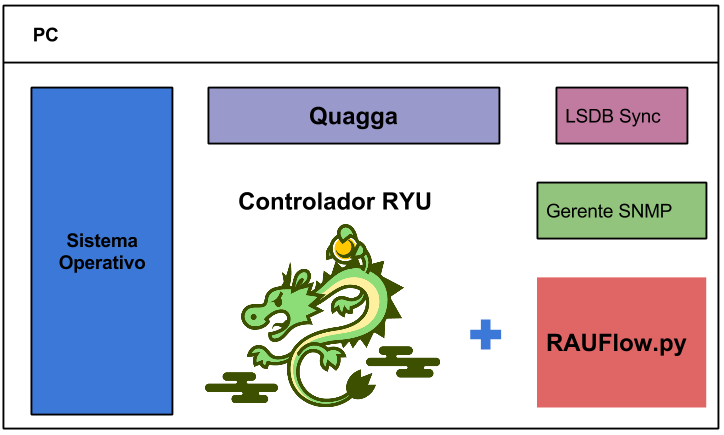
\includegraphics[width=0.6\textwidth]{Arch_Figure3}
\caption[OpenSourceRArch3]{Diagrama de componentes del Controlador}
\label{fig:OpenSourceRArch3}
\end{figure}

\section{Software de Control Ryu}
[yo]

\section{Quagga}
Como se menciona anteriormente, el Controlador ejecuta una instancia de Quagga. De esta forma tiene acceso local a la información de la base de datos topologica construida por OSPF.

\section{LSDB Sync}
LSDB Sync se encarga de tomar la información de la base de datos topologica una vez que el algoritmo ospf converge, procesarla y enviársela a las aplicaciones que se ejecutan en el software de control(Ryu), en este caso principalmente a la aplicación RAUFlow.\\

Esta componente consta de dos módulos. El primero se encarga de escuchar los mensajes del protocolo ospf que envia Quagga; generando un evento cuando ospf reconverge luego de producirse un cambio en la topologia, y es tomado por el segundo modulo.\\

Una vez capturado el evento anterior, el segundo m\'odulo toma la informacion topologica en la base local del Controlador y la procesa para ser enviada a la aplicación de control.

\section{Administrador SNMP}

El administrador SNMP es utilizado para consultar al agente snmp de un nodo en particular, por la correspondencia entre números de puerto OpenFlow y direcciones IP. Esta componente es utilizada por la aplicación de gestión RAUFlow cada vez que es preciso obtener esta información de mapeo para un nodo en particular(por ejemplo en el proceso de actualización de la topolog\'ia).

\section{Dise\~no general}

De esta forma, el prototipo para la nueva versi\'on de la red acad\'emica, se compone principalmente de algunos nodos construidos en base al router opensource, y un dispositivo controlador. Como se puede observar en la imagen \ref{fig:OpenSourceRArch4} los nodos se comunican con el Controlador mediante el protocolo OpenFlow como se explico con anterioridad, habilitando de esta forma a que el plano de datos sea programado por el plano de control. Por otro lado las diferentes instancias de Quagga distribu\'idas en cada nodo de la red y en el dispositivo controlador, se comunican mediante un canal IP con el objetivo de aprender la topolog\'ia y diseminar la informaci\'on de ruteo. Finalmente el gerente SNMP interactua con los diferentes agentes SNMP localizados en cada nodo mediante el canal IP, para obtener infirmaci\'on adicional acerca de cada nodo. 

\begin{figure}[htbp!] 
\centering    
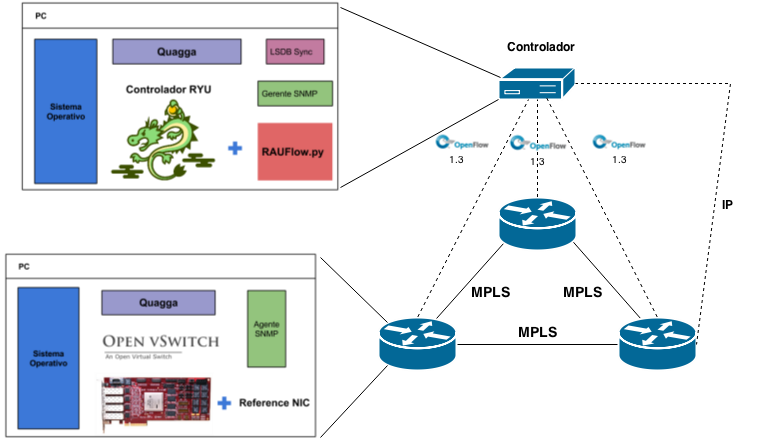
\includegraphics[width=0.9\textwidth]{Arch_Figure4}
\caption[OpenSourceRArch4]{Vista l\'ogica del prototipo}
\label{fig:OpenSourceRArch4}
\end{figure}